%Dies ist die Vorlage für die einzelnen Kapitel, die jeweils mit Chapter als Kapiteltitel starten
\chapter{Transportwegverschlüsselung}
Das \ac{SSL}-Protokoll wurde zunächst durch die Firma Netscape entwickelt, um die Kommunikation über \ac{HTTP}-Verbindungen abzusichern.\footcite[S. 796]{Eckert2013} \ac{SSL} kann auf der Sitzungs- und Präsentationsschicht des \ac{OSI}-Referenzmodells angesiedelt werden und setzt meist auf dem \ac{TCP} auf. Es hat die Aufgabe den darüber liegenden Schichten die Möglichkeit für eine authentifizierte, integritätsgeschützte und verschlüsselte Kommunikation zu geben.\footcite[Vgl.][S. 799 ff.]{Eckert2013}
Die Version \ac{SSL} 3.0 hat sich mittlerweile als de facto Standard im Internet durchgesetzt und wird von allen gängigen Browsern unterstützt.

Das \ac{TLS}-Protokoll kann als Weiterentwicklung von \ac{SSL} 3.0 angesehen werden und liegt aktuell in der Version 1.2 vor.
Da beide Protokolle in ihren Kernkonzepten übereinstimmen werden sie häufig synonym verwandt. Da \ac{TLS} jedoch eine Weiterentwicklung von \ac{SSL} ist, werden dort einige Erweiterungen eingeführt sowie unsichere Verfahren zur Berechnung von \ac{MAC}-Werten durch neuere Varianten ersetzt.\\
\begin{wrapfigure}{r}{0.5\textwidth}
	\begin{center}
		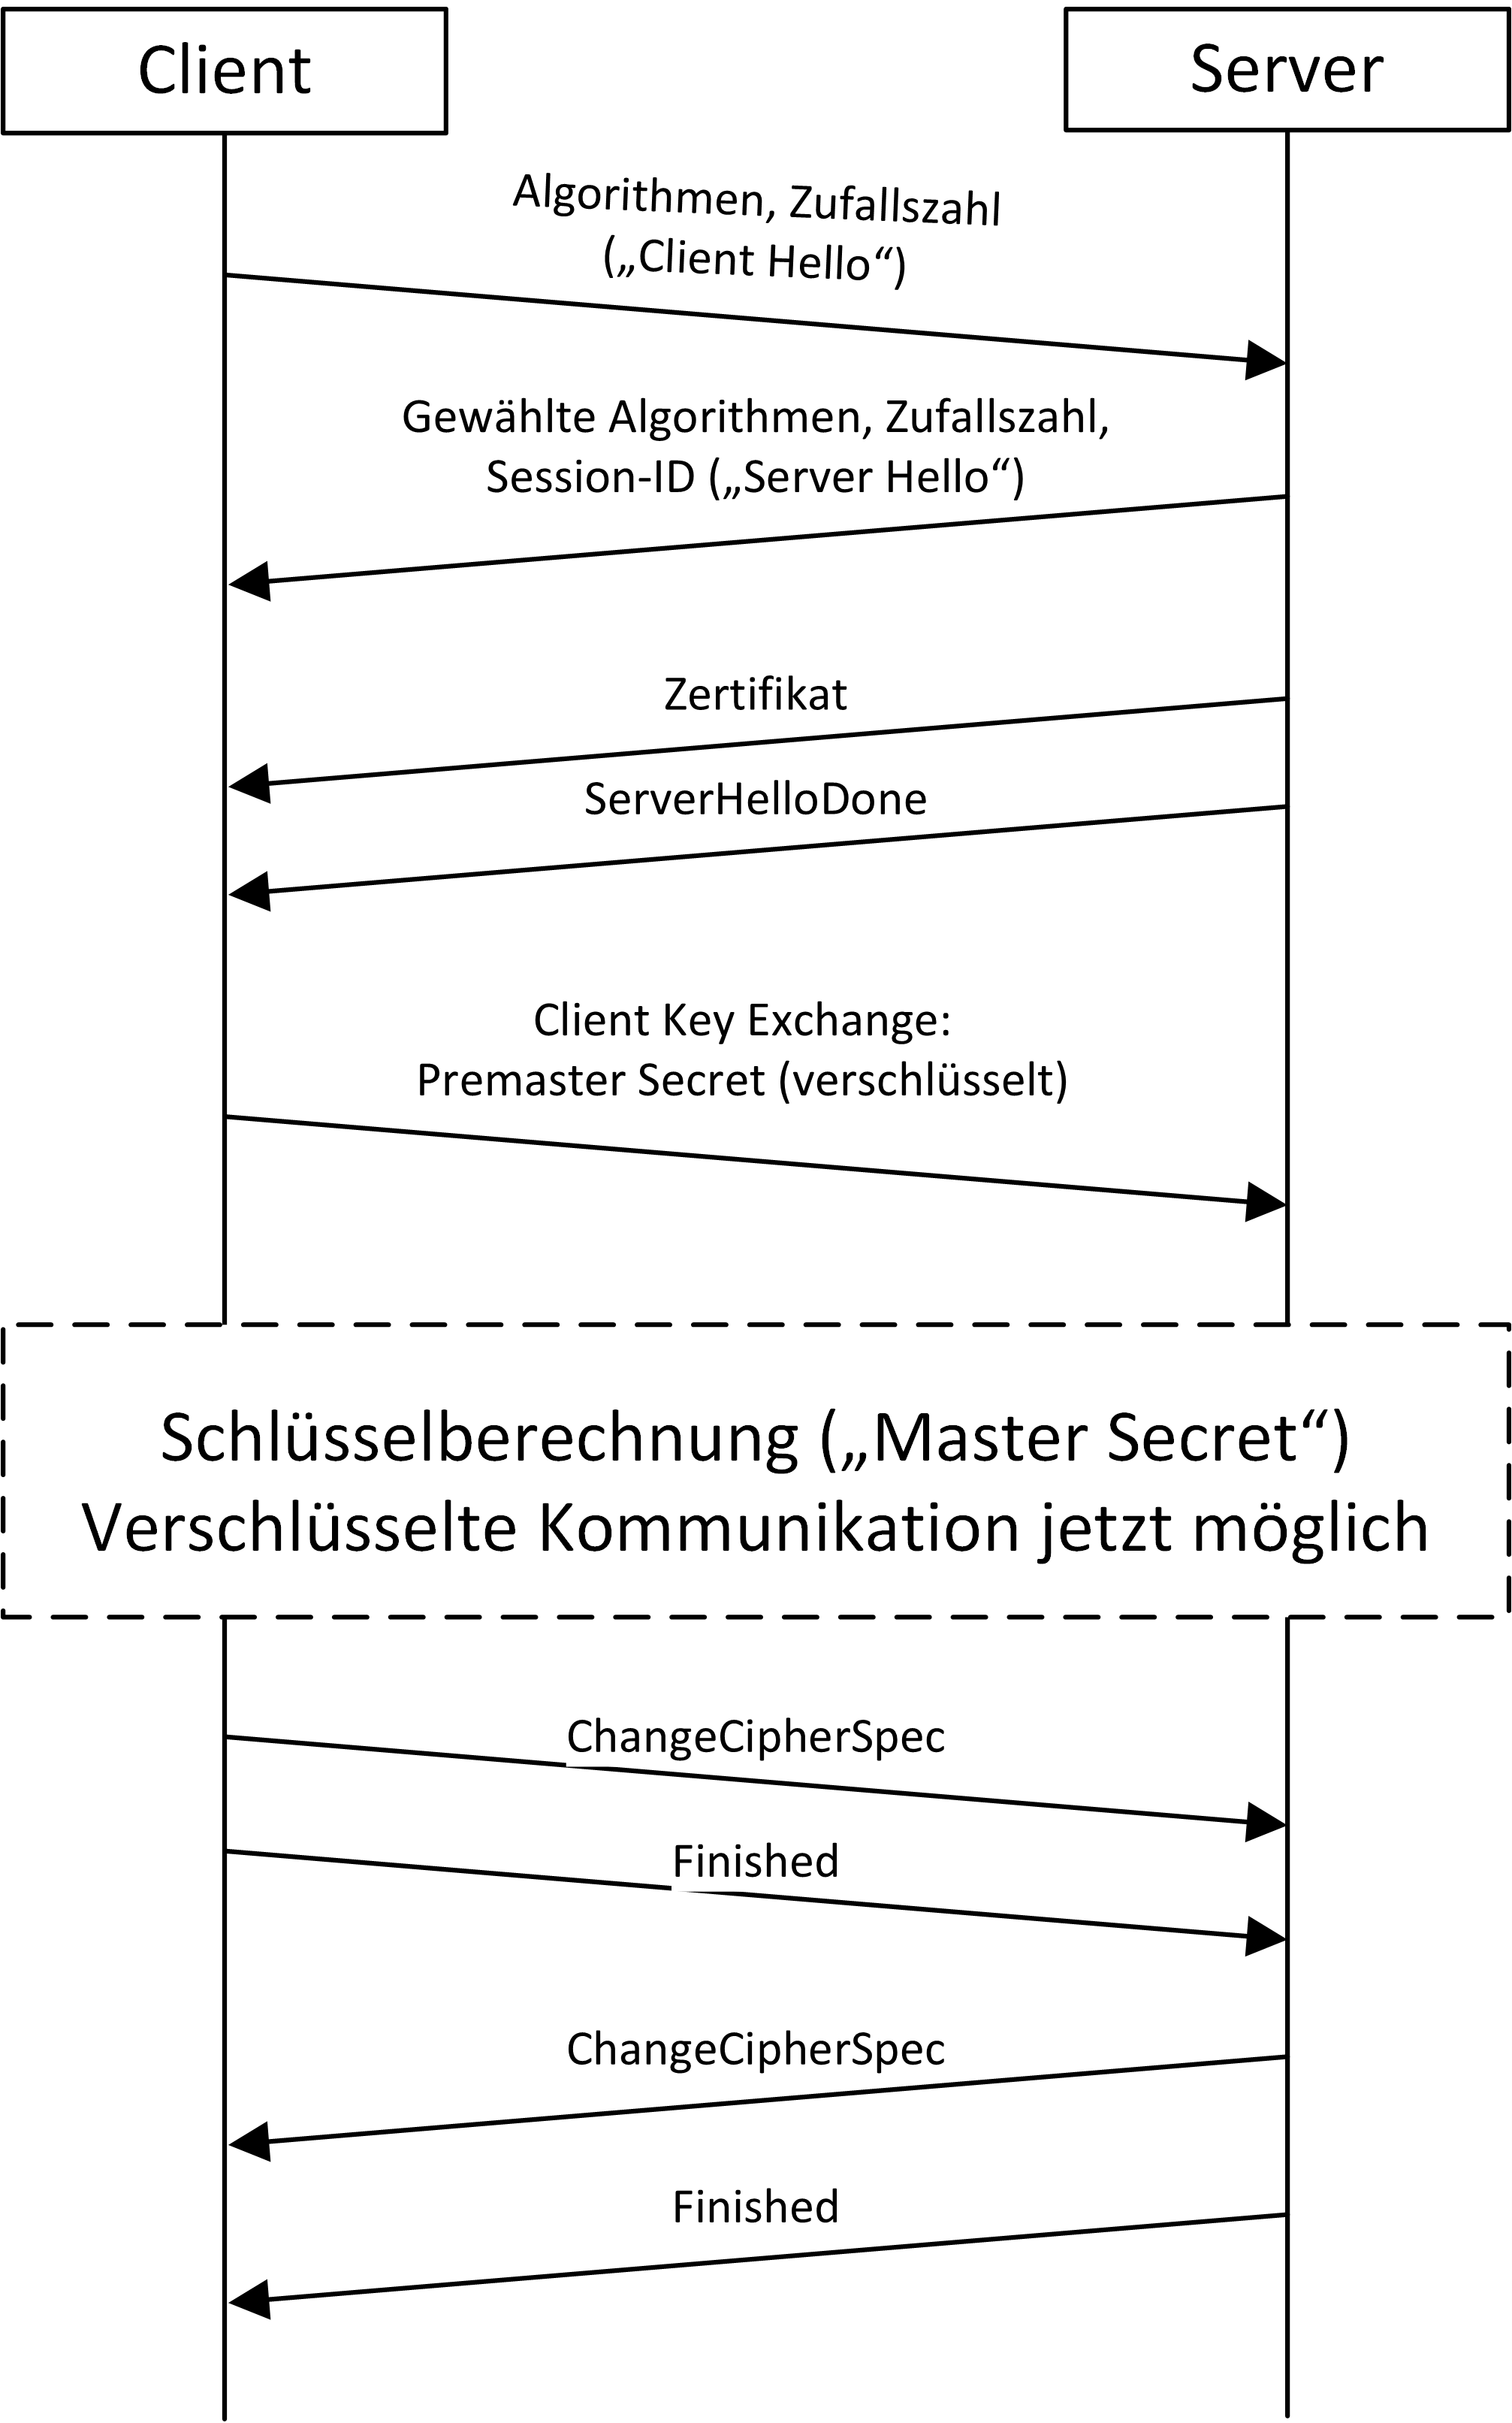
\includegraphics[width=0.4\textwidth]{images/MSC_Transport.png}
	\end{center}
	\caption{Handshake-Protokoll mit RSA}
	\footcite[In Anlehnung an][S. 170]{Sorge2013}
	\label{MSC_Transport}
\end{wrapfigure}

Beide Protokolle bestehen aus mehreren Schichten bzw. Unterprotokollen wobei das Record- und das Handshakeprotokoll von besonderer Bedeutung sind. 
Das Record-Protokoll ist für die Fragmentierung, Authentifizierung mittels \ac{MAC} und Verschlüsselung der zu übertragenden Daten zuständig. 
Mittels des Handshakeprotokolls werden Sitzungen zwischen den Kommunikationspartnern hergestellt. 
Dies bedeutet, dass die Kommunikationspartner durch den Austausch von Zertifikaten authentifiziert werden können und alle Informationen, die zur Berechnung des Shared Secret für die symmetrische Verschlüsselung der Daten benötigt werden, ausgetauscht werden. 
Die folgende Abbildung verdeutlicht den schematischen Ablauf eines solchen Sitzungsaufbaus unter Verwendung von \ac{RSA} für den Schlüsselaustausch.

Durch die flexible Gestaltung des Handshake-Protokolls wird gleichzeitig auch die Komplexität von \ac{TLS/SSL} stark erhöht. 
Dies hat zur Folge, dass durch die hohe Komplexität nicht mit Sicherheit alle Schwachstellen beim Design des Protokolls entfernt werden konnten. 
Außerdem ist zu bedenken, dass \ac{TLS/SSL} aufgrund seiner weiten Verbreitung ein lohnendes Ziel für Angriffe ist. Die Sicherheit des Protokolls hängt dabei stark von den genutzten kryptologischen Methoden ab. 
Außerdem ist zu beachten, dass es sich, aufgrund der Ansiedlung des Protokolls unterhalb der Anwendungsschicht, nur um eine Verschlüsselung der transportierten Nutzdaten auf dem Transportweg handelt. 
Die Daten werden am Kommunikationsendpunkt entschlüsselt und anschließend an die entsprechende Anwendung weitergereicht.

Auch die Authentifizierung der Kommunikationspartner mittels Zertifikaten weißt dieselben Schwachstellen durch die Vertrauensbeziehung zu bekannten \ac{CA}s, die unzureichend gesichert sind, auf.  